% 15. Составьте функциональную схему и опишите функциональные связи между подсистемами в составе системы, а также между подсистемами и внешней средой, которые Вы предполагаете учитывать при разработке математической модели системы.
% 16. Какую систему (или системы) Вы готовы рассматривать как актуальный прототип по отношению к системе, рассматриваемой в Вашей работе?
% 17. Какую задачу – анализа или синтеза системы – Вы решаете? Как решаемая задача связана с целью Вашего исследования?
% 18. Укажите тип математической модели (аналитическая, основанная на использовании физических законов и/или теории, имитационная, эмпирическая), которую Вы будете использовать для решения задачи анализа системы.
% 19. Охарактеризуйте кратко особенности разрабатываемой Вами модели системы.
% 20. В каком состоянии находится разработка модели в настоящее время?
% 21. В какой среде программирования Вы реализуете модель системы?
% 22. Если в работе решается задача синтеза системы, то какой алгоритм оптимизации альтернативы системы Вы используете или предполагаете использовать?
% 23. Если при синтезе системы рассматриваются несколько показателей ее эффективности, то как решается задача оптимизации системы по векторному критерию?

Попытки описания механизмов, позволяющих реализовать разделение функционала уже существуют в наше время. Пример - спецификация OSGI, которая лежит в основе IDE Eclipse и называется Equenox.

Спецификация OSGI предполагает построение (синтез) системы из обособленных компонентов. Для разделения зависимостей на сторонние библиотеки и сервисы. Степень разделения и ее характер зависит от реализации. В IDE Eclipse она реализована для решения целей и задач стоящих перед самой IDE, однако предполагает ее расширение по правилам конкретного бизнеса.

Так, в своей работе мне необходимо выработать, сформировать распределение заданного множества требований реализованных в файлах исходного кода по плагинам для достижения конкурентоспособности бизнеса по ранее описанным критериям.

Для этого я разработал графовую модель, в которую вошли выявленные сущности предметной области с характерными им ограничениями. Как один из этапов, она решает задачу разрешения циклических зависимостей между файлами исходного кода для построения графа трассируемости требований к ПО на файлы исходного кода. Благодаря этому достигается сокращение сущностей на слое файлов исходного кода за счет слияние циклически зависимых вершин графа в одну вершину и, как следствие, упрощается задача распределения файлов по плагинам.

На языке программирования Java написан решение обозначенной задачи, получены результаты экспериментов для оценки времени работы приложения от типа используемых коллекций, в которых хранится информация о графе:
\begin{enumerate}
    \item вершины - файлы исходного кода и требования к ПО;
    \item ребра - зависимости между файлами исходного кода и трассируемость требований к ПО.
\end{enumerate}

Работа алгоритма заключается в итеративном поиске циклов в графе с последующим слиянием входящем в цикл вершин до тех пор, пока в графе не будут отсутствовать циклы.

Схема работы разработанного решения приведена на рисунке \ref{fig:application_scheme}.

\begin{figure}[H]
    \centering
    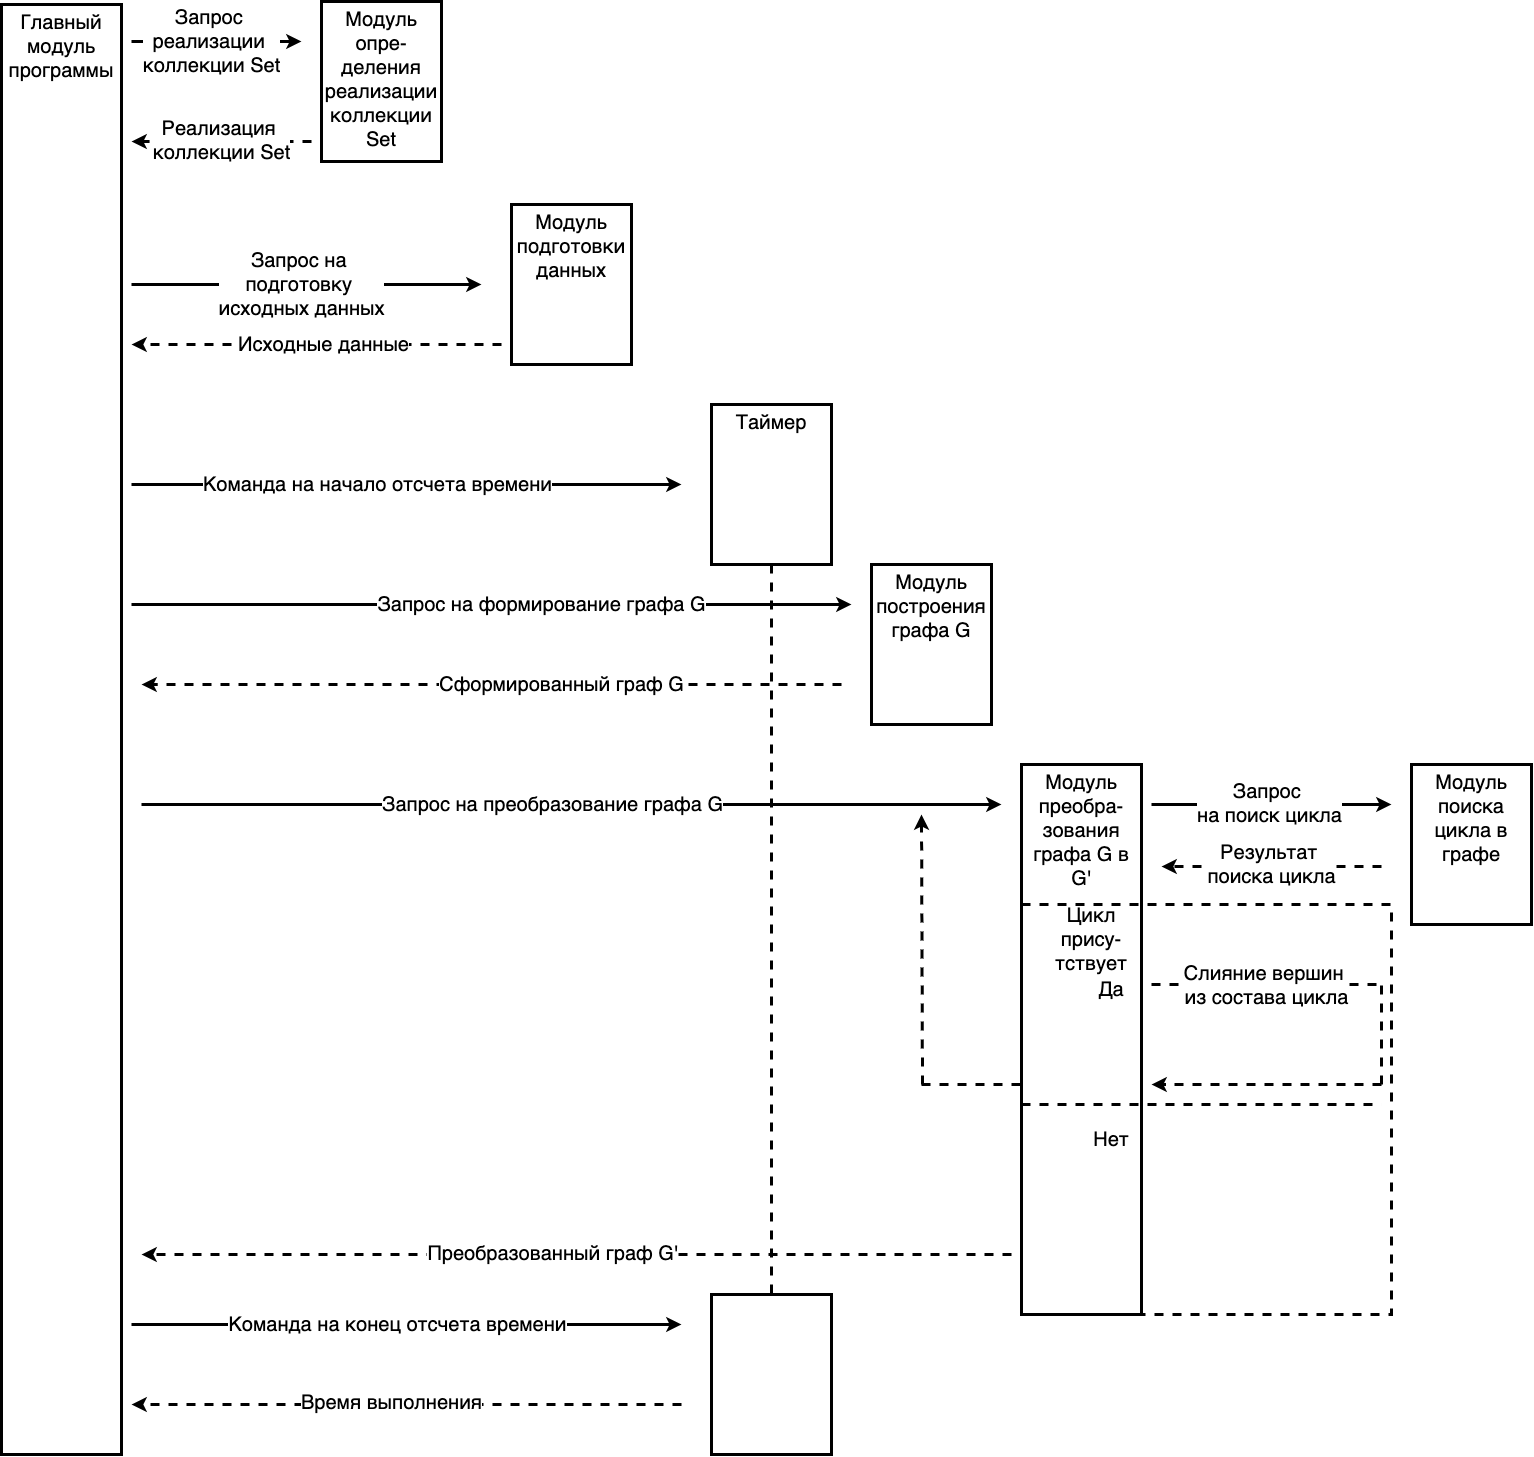
\includegraphics[width=1\textwidth]{application_scheme}
    \caption{Схема разработанного решения}
    \label{fig:application_scheme}
\end{figure}

В дальнейшем предполагается доработка модели для поиска оптимального распределения файлов исходного кода по плагинам при заданных ограничениях на систему, например обособление по частоте вызовов функций при числе плагинов не более пяти единиц.

Решение этой задачи предполагается выполнять с применением таких алгоритмов как:
\begin{enumerate}
    \item генетический алгоритм;
    \item PageRank;
    \item решающий лес;
\end{enumerate}

После решения этой задачи различными подходами будет произведена оценка полученных результатов и сделан вывод о том, при каких начальных условиях или их диапазонах лучше применять тот или иной алгоритм для решения задачи оптимальной декомпозиции.

Поиск оптимального решения предполагает введения ценовых коэффициентов или задание целевых функций вычисления стоимости сформированного алгоритмом оптимизации решения. Таким образом будет достигнута возможность проведения объективной оценки результата работы того или иного алгоритма.